\documentclass[14pt, a4paper]{article}
\usepackage[russian]{babel}
\usepackage{graphicx}
% \usepackage{tabularx}
\usepackage{layout}
\usepackage[14pt]{extsizes}
\usepackage[hidelinks]{hyperref}
\usepackage{caption}

\usepackage{listings}
\usepackage{xcolor}
\usepackage{float}

\setcounter{tocdepth}{4}
\setcounter{secnumdepth}{4}
\setlength{\emergencystretch}{2pt}
% \usepackage[compact]{titlesec}

\oddsidemargin = 0pt
\marginparwidth = 45pt %57
\textwidth = 467pt
\textheight = 716pt
\topmargin = 0pt %17
\footskip = 30pt %30
\headheight = 0pt %12
\headsep = 0pt %25

\title{Методичка 4}

\definecolor{codegreen}{rgb}{0,0.6,0}
\definecolor{codegray}{rgb}{0.5,0.5,0.5}
\definecolor{codepurple}{rgb}{0.58,0,0.82}
\definecolor{backcolour}{rgb}{0.97,0.97,0.97}

\lstdefinestyle{mystyle}{
    backgroundcolor=\color{backcolour},   
    commentstyle=\color{codegreen},
    keywordstyle=\color{magenta},
    numberstyle=\tiny\color{codegray},
    stringstyle=\color{codepurple},
    basicstyle=\ttfamily\footnotesize,
    breakatwhitespace=false,         
    breaklines=true,                 
    captionpos=b,                    
    keepspaces=true,
    frame=single,                 
    % numbers=left,                    
    % numbersep=5pt,                  
    showspaces=false,                
    showstringspaces=false,
    showtabs=false,                  
    tabsize=2,
    extendedchars=\true,
    inputencoding=utf8x
}

\lstset{style=mystyle}


\begin{document}

\begin{titlepage}
    \topmargin=216pt
    \newpage
    \hangindent=0.7cm
    \huge ИУ-10\\
    Системное\\
    Программное\\
    Обеспечение\\
    \textbf{Как работает nginx}

    \vspace{10cm}

    \begin{center}
        \small\textit{Москва, 2022}
    \end{center}
\end{titlepage}\newpage

\tableofcontents
\newpage

\begin{figure}[h]%current location
    \centering
    \scalebox{1}{
\includegraphics[width=0.8\textwidth]{imgs/1.0.png}}
    \label{1.0}
\end{figure}

\section*{Проблемы Apache}
\addcontentsline{toc}{section}{Проблемы Apache}

Веб-сервер Apache до сих пор занимает видное место в интернете. Корни этого проекта уходят в начало 
1990-х годов, и изначально его архитектура была заточена под существовавшие тогда системы и аппаратное 
обеспечение, а также общую степень развития интернета. Тогда веб-сайт, как правило, представлял из себя 
отдельный физический сервер, на котором работал единственный экземпляр Apache. К началу двухтысячных 
стало очевидно, что модель с единственным физическим сервером не может быть эффективно реплицирована 
для удовлетворения нужд растущих веб-сервисов. Несмотря на то, что Apache является неплохой 
платформой для дальнейших разработок, изначально он был спроектирован для создания копии веб-сервера 
для каждого нового соединения, что в современных условиях не позволяет добиться необходимой масштабируемости.

В конечном счете вокруг Apache развилась мощная экосистема сторонних сервисов, 
что позволяет разработчикам получать практически любые инструменты для создания приложений. 
Но у всего есть цена, и в данном случае за большое количество инструментов для работы с 
единственным программным продуктом, необходимо расплачиваться меньшими возможностями масштабирования.

Традиционные основанные на работе с потоками или процессами модели обработки одновременных соединений 
подразумевают обработку каждого соединения с помощью отдельного процесса или потока и блокирование 
операций ввода/вывода. В зависимости от приложения такой подход может быть крайне неэффективным с 
точки зрения затрат ресурсов процессора и памяти. Создание отдельного процесса или потока требует 
подготовки новой среды запуска, включая выделение памяти стека и кучи, а также создания нового 
контекста выполнения. На все это тратится дополнительное процессорное время, что в итоге может 
приводить к проблемам с производительностью из-за избыточных переключений контекста. Все эти 
проблемы в полной мере проявляются при использовании веб-серверов старой архитектуры, таких как Apache.

\section*{Обзор архитектуры веб-сервера nginx}
\addcontentsline{toc}{section}{Обзор архитектуры веб-сервера nginx}
С самого начала своего существования \textbf{nginx} должен был играть роль специализированного инструмента, 
позволяющего достичь более высокой производительности и экономичности использования серверных ресурсов, 
одновременно позволяя осуществлять динамический рост веб-сайта. В итоге \textbf{nginx} получил асинхронную, 
модульную, событийно-ориентированную архитектуру.

\textbf{Nginx} активно использует мультиплексирование и нотификации событий, назначая конкретные задачи 
отдельным процессам. Соединения обрабатываются с помощью эффективного цикла выполнения с помощью 
определенного количества однопоточных процессов, называемых worker’ами. Внутри каждого \textbf{worker} 
\textbf{nginx} может обрабатывать многие тысячи одновременных соединений и запросов в секунду.


\section*{Структура кода}
\addcontentsline{toc}{section}{Структура кода}

\textbf{Worker} в \textbf{nginx} включает ядро и функциональные модули. Ядро nginx отвечает за поддержание 
цикла выполнения и исполнения подходящих секций кода модулей на каждом шаге обработки процесса. 
Модули предоставляют большую часть функциональности уровня приложений. Также модули читают и 
пишут в сеть и хранилище, трансформируют контент, осуществляют исходящую фильтрацию и, в случае 
работы в режиме прокси, передают запросы вышестоящим серверам.

Модульная архитектура \textbf{nginx} позволяет разработчикам расширять набор функций веб-сервера 
без необходимости модификации кода его ядра. Существует несколько разновидностей модулей 
\textbf{nginx} — модули ядра, модули событий, фазовые обработчики, протоколы, фильтры, балансировщики 
нагрузки, обработчики переменных и т.п. При этом \textbf{nginx} не поддерживает динамически загружаемые 
модули, то есть они компилируются вместе с ядром на стадии создания сборки. Разработчики планируют 
добавить функциональность загружаемых модулей в будущем.

Для организации различных действий, связанных с приемом, обработкой и управлением сетевыми 
соединениями и загрузкой контента, \textbf{nginx} использует механизмы нотификаций и несколько механизмов 
улучшения производительности дискового ввода/вывода в \textbf{ОС Linux}, \textbf{Solaris} и \textbf{BSD-системах} — среди 
них \textbf{kqueue}, \textbf{epoll} и \textbf{event ports}.

Высокоуровневое представление архитектуры nginx показано на рисунке ниже:
\begin{figure}[h]%current location
    \centering
    \scalebox{1}{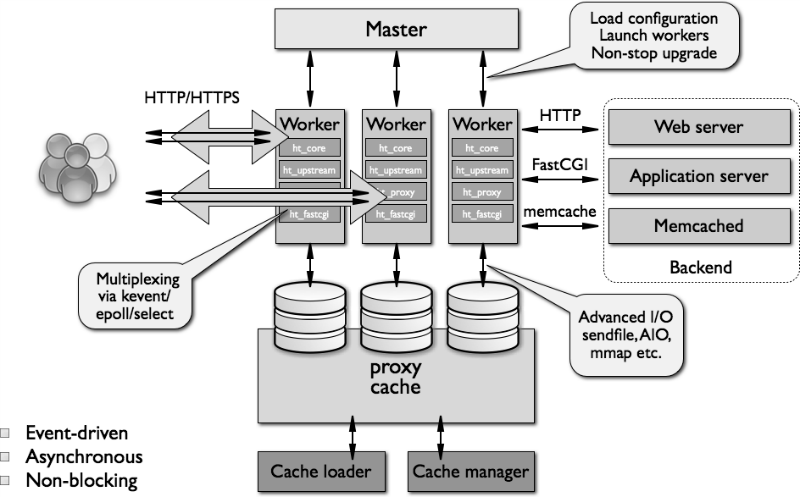
\includegraphics[width=0.8\textwidth]{imgs/1.1.png}}
    \label{1.1}
\end{figure}



\section*{Модель работы worker-процессов}
\addcontentsline{toc}{section}{Модель работы worker-процессов}
Как было отмечено выше, \textbf{nginx} не создает процесс или поток для каждого соединения. 
Вместо этого специальный \textbf{worker} обрабатывает прием новых запросов с общего «слушающего» 
сокета и запускает высокоэффективный цикл выполнения внутри каждого \textbf{worker}-процесса — это 
позволяет обрабатывать тысячи соединений для одного \textbf{worker’а}. Каких-то специальных механизмов 
распределения соединений между разными \textbf{worker}-процессами в \textbf{nginx} нет, эта работа выполняется 
в ядре \textbf{ОС}. В процессе загрузки создается набор слушающих сокетов, а затем worker постоянно 
принимает, считывает и пишет в сокеты в процессе обработки HTTP-запросов и ответов.

Самой сложной частью кода «воркеров» \textbf{nginx} является описание цикла выполнения. 
Он включает всевозможные внутренние вызовы и активно использует концепцию асинхронной 
обработки задач. Асинхронные операции реализованы посредством модульности, оповещений о 
событиях, а также широкого использования колбэк-функций и доработанных таймеров. Главная 
цель всего этого — по максимуму уйти от использования блокировок. Единственным случаем, 
когда \textbf{nginx} может их применять, является ситуация недостаточной для работы \textbf{worker}-процесса 
производительности дискового хранилища.

Поскольку \textbf{nginx} не создает процессы и потоки для каждого соединения, в подавляющем большинстве 
случаев веб-сервер очень консервативно и крайне эффективно работает с памятью. Кроме того, он 
сохраняет циклы процессора, поскольку в случае \textbf{nginx} отсутствует паттерн постоянного создания 
и уничтожения процессов и потоков. \textbf{Nginx} проверяет состояние сети и хранилища, инициализирует 
новые соединения, добавляет их в цикл выполнения, а затем асинхронно обрабатывает до «победного 
конца», после чего соединение деактивируется и исключается из цикла. Благодаря этому механизму, 
а также вдумчивому использованию системных вызовов и качественной реализации поддерживающих 
интерфейсов вроде распределителей памяти (\textbf{pool} и \textbf{slab}), \textbf{nginx} позволяет добиться низкой или 
средней загрузки \textbf{CPU} даже в случае экстремальных нагрузок.

Использование нескольких \textbf{worker}-процессов для обработки соединений также делает веб-сервер 
хорошо масштабируемым для работы с несколькими ядрами. Эффективное использование многоядерных 
архитектур обеспечивается созданием одного \textbf{worker}-процесса для каждого ядра, а также позволяет 
избежать блокировок и трешинга потоков. Механизмы контроля ресурсов изолированы внутри однопоточных 
worker-процессов — такая модель также способствует более эффективному масштабированию физических 
устройств хранения, позволяет добиваться более высокой утилизации дисков и избегать блокирования 
дискового ввода/вывода. В итоге ресурсы сервера используются эффективнее, а нагрузка распределяется
между несколькими worker-процессами.

Для разных паттернов загрузки процессора и диска число \textbf{worker}-процессов \textbf{nginx} может изменяться.
Разработчики веб-сервера рекомендуют системным администраторам пробовать различные варианты конфигурации, 
чтобы получить наилучшие результаты в плане производительности. Если паттерн можно описать как 
«интенсивную загрузку \textbf{CPU}» — например, в случае обработки большого количества \textbf{TCP/IP}-соединений, 
осуществления компрессии или использовании \textbf{SSL}, то число «воркеров» должно совпадать с количеством 
ядер. Если же нагрузка в основном падает на дисковую систему — например, при необходимости загрузки 
и выгрузки из хранилища крупных объёмов контента — то число worker-процессов может быть в полтора-два 
раза больше количества ядер.

В следующих версиях веб-сервера разработчики \textbf{nginx} планируют решить проблему возникновения ситуаций 
блокировки дискового \textbf{I/O}. На момент написания этой главы в случае недостаточной производительности 
хранилища при осуществлении дисковых операций конкретного \textbf{worker}-процесса, для него может быть 
заблокирована возможность чтения или записи. Чтобы свести такую вероятность к минимуму, можно 
использовать различные комбинации директив конфигурационных файлов и существующих механизмов — например,
опции \textbf{sendfile} и \textbf{AIO} обычно позволяют серьезно повысить производительность хранилища.

Еще одна проблема существующей модели worker-процессов связана с ограниченной поддержкой встроенных 
скриптов. В случае стандартной версии \textbf{nginx} доступно лишь встраивание \textbf{Perl}-скриптов. Такая ситуация 
объясняется просто — главной проблемой является вероятность того, что встроенный сценарий будет 
заблокирован в ходе выполнения операции или неожиданно завершится. В обоих случаях \textbf{worker}-процесс 
зависнет, что может затронуть тысячи соединений разом.

\section*{Роли процессов nginx}
\addcontentsline{toc}{section}{Роли процессов nginx}
\textbf{Nginx} запускает несколько процессов в памяти — один \textbf{master}-процесс и несколько «\textbf{воркеров}». 
Также существует несколько служебных процессов — например, менеджер и загрузчик кэша. В версиях 
\textbf{nginx 1.x} все процессы однопоточные. Все они используют для взаимодействия друг с другом механизмы 
разделения памяти. Master-процесс запускается под пользователем \textbf{root}. Служебные и worker-процессы 
работают без привилегий суперпользователя.

\textbf{Master}-процесс отвечает за следующие задачи:
\begin{itemize}
    \item чтение и валидация конфигурации;
    \item создание, связывание и закрытие сокетов;
    \item старт, прерывание и поддержка сконфигурированного количества worker-процессов;
    \item реконфигурация без прерывания работы сервиса;
    \item контроль постоянных двоичных обновлений (запуск новых «бинарников» и откат на предыдущую версию 
    в случае необходимости);
    \item повторное открытие лог-файлов;
    \item компиляция встроенных Perl-скриптов.
\end{itemize}
\begin{figure}[H]%current location
    \centering
    \scalebox{1}{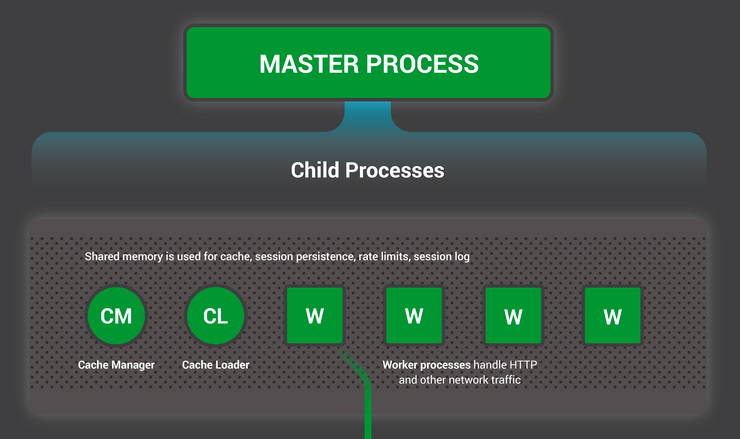
\includegraphics[width=0.8\textwidth]{imgs/1.2.png}}
    \label{1.2}
\end{figure}
\textbf{Worker}-процессы принимают и обрабатывают поступающие от клиентов соединения, предоставляют 
функциональность \textbf{reverse proxy} и фильтрации, а также делают почти все, что должен делать nginx. 
В общем случае, чтобы отследить текущее состояние веб-сервера, системному администратору нужно 
взглянуть на воркеры, поскольку именно они его [состояние] лучше всего отражают.

Процесс загрузчика кэша отвечает за проверку элементов, находящихся в кэше на диске, а 
также за обновление размещенной в памяти базы метаданными. Загрузчик готовит экземпляры 
nginx к работе с уже хранящимися на диске файлами. Он проходит по директориям, изучает 
метаданные контента в кэше, обновляет необходимые элементы в разделяемой памяти, а затем завершает работу.

Менеджер кэша главным образом отвечает за контроль актуальности кэша. При нормальном 
функционировании веб-сервера он находится в памяти, а в случае сбоя его перезапускает \textbf{master}-процесс.

\section*{Краткий обзор кэширования в nginx}
\addcontentsline{toc}{section}{Краткий обзор кэширования в nginx}
В \textbf{nginx} кэширование реализовано в форме иерархического хранилища данных в файловой системе. 
Ключи кэша могут быть сконфигурированы, и контролировать, что попадает в него, можно с 
помощью различных параметров запросов. Ключи кэша и метаданные хранятся в сегментах разделяемой 
памяти, к которым есть доступ у воркеров, а также у загрузчика и менеджера кэша. В настоящий 
момент в \textbf{nginx} нет кэширования файлов во внутренней памяти, кроме тех возможностей оптимизации, 
которые доступны при работе с механизмами виртуальной файловой системы ОС. Каждый закэшированный 
ответ помещается в отдельный файл файловой системы. Иерархия котролируется с помощью конфигурационных 
директив \textbf{nginx}. Когда ответ записывается в структуру директорий кэша, путь и имя файла извлекаются 
из \textbf{MD5}-хеша прокси-\textbf{URL}.

Процесс помещения контента в кэш проходит следующим образом: когда \textbf{nginx} считывает ответ 
с вышестоящего сервера, контент сначала записывается во временный файл вне структуры 
директорий кэша. Когда веб-сервер заканчивает обработку запроса, он меняет имя временного 
файла и перемещает его в директорию кэша. Если директория временных файлов размещается на 
другой файловой системе, то файл будет скопирован, поэтому рекомендуется размещать временную 
и кэш-директорию на одной файловой системе. Кроме того, с точки зрения безопасности хорошим 
решением в случае необходимости очистки файлов будет и их удаление из кэша, поскольку существуют 
сторонние расширения для nginx, которые могут предоставлять удаленный доступ к кэшированному контенту.


\section*{Конфигурация nginx}
\addcontentsline{toc}{section}{Конфигурация nginx}
На создание конфигурационной системы \textbf{nginx} Игоря Сысоева вдохновил опыт работы с \textbf{Apache}. 
Разработчик считал, что для веб-сервера необходима масштабируемая конфигурационная система.
И главная проблема масштабируемости возникала при необходимости поддержки большого количества 
сложных конфигураций с множеством виртуальных серверов, директорий и наборов данных. Поддержка 
и масштабирование относительно крупной веб-инфраструктуры может превратиться в настоящий ад.

В результате конфигурация \textbf{nginx} была спроектирована таким образом, чтобы упростить рутинные 
операции по поддержке веб-сервера и предоставить инструменты для дальнейшего расширения системы.

Конфигурация \textbf{nginx} хранится в нескольких текстовых файлах, которые обычно располагаются в 
директориях \textbf{/usr/local/etc/nginx} или \textbf{/etc/nginx}. Главный конфигурационный файл обычно называется \linebreak
\textbf{nginx.conf}. Чтобы сделать его более читабельным, части конфигурации можно разнести по разным файлам, 
которые затем включаются в главном. При этом важно заметить, что \textbf{nginx} не поддерживает файлы 
\textbf{.htaccess} — вся конфигурационная информация должна располагаться в централизованном наборе файлов.

Изначальное чтение и проверка конфигурационных файлов осуществляется \textbf{master}-процессом. 
Скомпилированная форма конфигурации для чтения доступна \textbf{worker}-процессам после их выделения 
из \textbf{master}-процесса. Конфигурационные структуры автоматически разделяются механизмами управления виртуальной памятью.

Существует несколько различных контекстов для блоков и директив \textbf{main, http, server, 
upstream, location (mail, для mail proxy)}. К примеру, нельзя поместить блок \textbf{location} в 
блок директив \textbf{main}. Также, чтобы не добавлять лишнюю сложность, в \textbf{nginx} 
нет конфигурации «глобального веб-сервера». 

Как говорит сам Сысоев:

Локации, директории и другие блоки в конфигурации глобального веб-сервера — это то, 
что мне никогда не нравилось в \textbf{Apache}, поэтому они никогда не появлялись в \textbf{nginx}.

Синтаксис и форматирование конфигурации \textbf{nginx} следуют стандарту оформления кода \textbf{C} 
\textbf{(“C-style convention”)}. 
Несмотря на то, что некоторые директивы \textbf{nginx} отражают определенные части конфигурации\linebreak \textbf{Apache}, 
в целом настройка двух веб-серверов серьезно отличается. К примеру, в \textbf{nginx} поддерживаются 
правила перезаписи, а в случае Apache для этого администратор вручную должен будет адаптировать 
\textbf{legacy}-конфигурацию. Различается и реализация «движка» перезаписи.

\textbf{Nginx} также поддерживает несколько полезных оригинальных механизмов. К примеру — переменные 
и директива \textbf{try\_files}. В \textbf{nginx} переменные используются для реализации мощного механизма 
контроля \textbf{run-time}-конфигурации веб-сервера. Они могут использоваться с различными 
конфигурационными директивами для обеспечения дополнительной гибкости в описании условий обработки запросов.

Директива \textbf{try\_files} изначально создавалась в качестве замены условных операторов \textbf{if}, а также для 
быстрого и эффективного сопоставления разных \textbf{URL} и контента.

\section*{Внутреннее устройство nginx}
\addcontentsline{toc}{section}{Внутреннее устройство nginx}
\textbf{Nginx} состоит из ядра и целого ряда модулей. Ядро отвечает за создание основы веб-сервера, 
работу функциональности \textbf{web-} и \textbf{reverse}-прокси. Также оно отвечает за использование сетевых 
протоколов, построение среды запуска и обеспечение беспроблемного взаимодействия между разными 
модулями. Однако большая часть функций, связанных с протоколами и приложениями, реализуется с 
помощью модулей, а не ядра.

Соединения обрабатываются \textbf{nginx} с помощью трубы или цепи модулей. Другими словами, для 
каждой операции есть модуль, который выполняет нужную работу — например, компрессию, 
модификацию контента, выполнение серверных включений, взаимодействие с внешними серверами 
через \textbf{FastCGI} или \textbf{uwsgi}-протоколы, или общение с \textbf{memcahed}.

Существует пара модулей, которые размещаются между ядром и «функциональными» модулями — это 
\textbf{http} и \textbf{mail}-модули. Они обеспечивают дополнительный уровень абстракции между ядром и 
низкоуровневыми компонентами. С их помощью реализована обработка последовательностей 
событий, связанных с определенным сетевым протоколом вроде \textbf{HTTP}, \textbf{SMTP} или \textbf{IMAP}. Вместе 
с ядром эти высокоуровневые модули отвечают за поддержание верного порядка вызовов 
соответствующих функциональных модулей. В настоящий момент \textbf{HTTP}-протокол реализован 
в качестве части \textbf{http}-модуля, однако в будущем разработчики планируют выделить его в 
отдельный функциональный модуль — это продиктовано необходимостью поддержки других протоколов (например, SPDY).

Большинство существующих модулей дополняют \linebreak\textbf{HTTP}-функциональность \textbf{nginx}, но модули событий и 
протоколов также используются и для работы с почтой (mail). Модули событий предоставляют 
механизм оповещений о событиях для различных ОС — например, \textbf{kqueue} или \textbf{epoll}. Выбор модуля, 
используемого nginx, зависит от конфигурации сборки и возможностей операционной системы. 
Модули протоколов позволяют \textbf{nginx} работать через \textbf{HTTPS}, \textbf{TLS/SSL}, 
\textbf{SMTP}, \textbf{POP3} и \textbf{IMAP}.

Вот так выглядит типичный цикл обработки HTTP-запроса:
\begin{enumerate}
    \item Клиент отправляет HTTP-запрос.
    \item Ядро в соответствии со сконфигурированной локацией для запроса nginx выбирает нужный фазовый обработчик.
    \item В случае включенной прокси-функциональности модуль балансировки нагрузки 
    выбирает для целей проксирования вышестоящий сервер.
    \item Фазовый обработчик заканчивает свою работу и передает буфер вывода первому фильтру.
    \item Первый фильтр передает вывод второму фильтру.
    \item Второй фильтр передает вывод третьему фильтру (и так далее).
    \item Итоговый ответ пересылается клиенту.
\end{enumerate}

Вызов модулей в nginx можно настраивать, он осуществляется с помощью колбэков с указателями на 
исполняемые функции. Минус здесь заключается в том, что если разработчик хочет написать собственный 
модуль, то ему нужно будет четко прописать, как и где он должен запускаться. К примеру, вот в каких 
точках это может происходить:
\begin{itemize}
    \item До чтения и обработки конфигурационного файла.
    \item В момент завершения инициализации главной конфигурации.
    \item После инициализации сервера (хоста/порта).
    \item Когда серверная конфигурация сливается с основной.
    \item Когда стартует или завершается master-процесс.
    \item В момент старта или завершения нового worker-процесса.
    \item В момент обработки запроса.
    \item В процессе фильтрации заголовка и тела ответа.
    \item При выборе начальной и повторной инициализации запроса к вышестоящему серверу.
    \item В процессе обработки ответа от вышестоящего сервера.
    \item В момент завершения взаимодействия с этим сервером.
\end{itemize}
Внутри воркера последовательность действий, ведущая в цикл обработки, где генерируется ответ, выглядит следующим образом:
\begin{itemize}
    \item Старт ngx\_worker\_process\_cycle().
    \item События обрабатываются с помощью механизмов ОС (например, epoll или kqueue).
    \item События принимаются, отправляются соответствующие действия.
    \item Процесс/прокси запрашивает заголовок и тело.
    \item Контент ответа (заголовок, ответ) генерируется и отправляется клиенту.
    \item Запрос финализируется.
    \item Таймеры и события повторно инициализируются.
\end{itemize}
Более детализированное описание обработки HTTP-запроса можно представить так:
\begin{enumerate}
    \item Инициализация обработки запроса.
    \item Обработка заголовка.
    \item Обработка тела.
    \item Вызов соответствующего обработчика.
    \item Прохождение фаз обработки.
\end{enumerate}
В процессе обработки запрос проходит несколько фаз. На каждой из них вызываются соответствующие 
обработчики. Обычно они выполняют четыре задачи: получают конфигурацию местоположения, генерируют 
соответствующий ответ, отправляют заголовок, а затем тело. У обработчика есть один аргумент: 
определенная структура, описывающая запрос. В структуре запроса содержится большое количество 
полезной информации: например, метод запроса, URL и заголовок.

После прочтения заголовка HTTP-запроса, nginx просматривает связанную конфигурацию виртуального 
сервера. Если виртуальный сервер найден, то запрос проходит шесть фаз:

\begin{enumerate}
    \item Фаза перезаписи сервера.
    \item Фраза поиска местоположения (location).
    \item Перезапись местоположения.
    \item Фаза контроля доступа (access control).
    \item Фаза работы try\_files.
    \item Фаза записи логов.
\end{enumerate}
В процессе создания контента в ответ на запрос, nginx передает его различным обработчикам 
контента. Сначала запрос может попасть к так называемым безусловным обработчикам вроде 
perl, proxy\_pass, flv, mp4. Если запрос не подходит ни к одному из этих обработчиков контента, 
то он по цепочке передается следующим обработчикам: random index, index, autoindex, gzip\_static, static.

Если специализированный модуль вроде mp4 или autoindex не подходит, то контент рассматривается в качестве 
директории на диске (то есть, в качестве статического) и за него отвечает контент-обработчик static.

После этого контент передается фильтрам, которые работают по определенной схеме. Фильтр получает вызов, 
начинает работать, вызывает следующий фильтр и так до момента вызова последнего фильтра в цепочке. 
Существуют фильтры заголовков и тела. Работа фильтра заголовка состоит из трех основных шагов:

\begin{enumerate}
    \item Определение необходимости действий в ответ на запрос.
    \item Обработка запроса.
    \item Вызов следующего фильтра.
\end{enumerate}
Фильтры тела трансформируют сгенерированный контент. Среди их возможных действий:
\begin{itemize}
    \item Серверные включения.
    \item Фильтрация XSLT.
    \item Фильтрация изображений (наример, ресайзинг картинок на лету).
    \item Модификация кодировки.
    \item Gzip-компрессия.
    \item Кодирование фрагментов (chunked encoding).
\end{itemize}
После прохождения цепочки фильтров ответ передается в модуль записи. Также существуют два специальных 
фильтра — copy и postpone. Первый из них отвечает за наполнение буферов памяти релевантным контентом 
ответов, а второй используется для подзапросов.

Подзапросы — это очень важный и очень мощный механизм для обработки запросов и ответов. 
С помощью подзапросов nginx может вернуть результат для разных URL, запрошенных клиентом. 
Некоторые веб-фреймворки для решения этой задачи используют внутренние редиректы, однако 
nginx идет дальше — фильтры не только выполняют разные подзапросы и комбинируют их вывод 
в один общий ответ, но подзапросы также могут быть иерархичными и вложенными. То есть 
подзапрос может выполнять собственный подзапрос («под-подзапрос»), а тот, в свою очередь, 
может инициировать «под-под-подзапрос».

Подзапросы могут указывать на файлы на диске, другие обработчики или вышестоящие серверы. 
Они крайне полезны для вставки дополнительного контента при использовании данных из 
первоначального запроса. К примеру, SSI-модуль (server side include) использует фильтр 
для парсинга содержимого возвращенного документа, а затем заменяет директивы include 
контентом из указанных URL-адресов. Точно так же можно создать фильтр, который превращает 
все содержимое документа в URL, а затем добавляет к URL сам новый документ.

Также в nginx есть модули балансировки нагрузки и upstream-модули. Последние используются 
для подготовки контента к отправки вышестоящему серверу и получения ответов от него. В 
этом случае не происходит вызовов фильтров вывода. Upstream-модуль устанавливает колбэки, 
которые нужно вызвать, когда вышестоящий сервер будет готов к записи или чтению. Существуют 
колбэки для реализации следующей функциональности:

\begin{itemize}
    \item Организация буфера запроса для отправки вышестоящему серверу.
    \item Повторная инициализация соединения с сервером (она происходит перед созданием запроса).
    \item Обработка первых битов ответа и сохранение указателей на данные, полученные с сервера.
    \item Прерывание запросов (происходит при неожиданном отключении клиента).
    \item Финализация запроса после того, как nginx закончит чтение с вышестоящего сервера.
    \item Обрезание тела ответа (удаление трейлера).
\end{itemize}
Модули балансировки нагрузки добавляются к обработчику proxy\_pass для обеспечения возможности 
выбора вышестоящего сервера — в случае, если их более одного. Механизмы работы с вышестоящими 
серверами и балансировки нагрузки позволяют выявлять неисправные серверы и перенаправлять запросы
к функционирующим узлам.

Также в nginx есть интересные модули, которые предоставляют дополнительный набор переменных для 
использования в конфигурационном файле. В nginx переменные главным образом создаются и обновляются 
в различных модулях, но есть и два модуля, которые целиком посвящены переменным: geo и map. Модуль 
geo используется для облегчения отслеживания клиентов по IP-адресам. Он может создавать случайные 
переменные, которые зависят от IP-адреса клиента. Второй модуль, map, позволяет создавать переменные 
из других переменных, что облегчает маппинг имен хостов и других runtime-переменных.

Механизмы распределения памяти в worker-процессах nginx были созданы с опорой на опыт Apache. 
Высокоуровневое описание работы с памятью в nginx звучит так: для каждого соединения необходимые 
буферы памяти динамически выделяются, линкуются и используются для хранения и изменения заголовка 
и тела запроса или ответа, а затем освобождаются при завершении соединения. Nginx пытается 
по-максимуму избегать копирования данных в памяти, большая часть из них обрабатывается с 
помощью переменных указателей без вызова memcpy.

Задача управления распределением памяти решается с помощью специального распределителя пула 
nginx. Зоны разделяемой памяти используются для приема мьютекс, метаданных кэша, кэша SSL-сессий 
и информации, связанной с управлением полосой пропускания (лимиты). Для управления распределением 
памяти в nginx реализован slab-распределитель. Безопасное использование разделяемой памяти 
осуществляется за счет механизмов блокировки (мьютексы и семафоры). Для организации сложных 
структур данных в nginx используется реализация красно-черных деревьев. Они применяются для 
сохранения метаданных кэша в разделяемой памяти, отслеживания не-regex определения местоположений 
и для некоторых других задач.

\end{document}